\documentclass[12pt]{article}
\usepackage{alltt}
\usepackage[utf8]{inputenc}
\usepackage[dvips]{graphicx}
%\usepackage{a4wide}
\usepackage{epsfig}
\usepackage{fancybox}
\usepackage{verbatim}
\usepackage{array}
\usepackage{latexsym}
\usepackage{alltt}
%\usepackage{dsfont}
\usepackage{caption}
\usepackage{subcaption}
%\usepackage{fullpage}
\usepackage{hyperref}
\usepackage{textcomp}
\usepackage{listings}
\usepackage{color}
\usepackage{amsmath}
\usepackage{amsfonts}
\usepackage{tikz}
\usepackage{float}
\usepackage{matlab-prettifier}
\usepackage{graphicx}

\usepackage[hmargin=3cm,vmargin=6.0cm]{geometry}
%\topmargin=0cm
\topmargin=-2cm
\addtolength{\textheight}{6.5cm}
\addtolength{\textwidth}{2.0cm}
%\setlength{\leftmargin}{-5cm}
\setlength{\oddsidemargin}{0.0cm}
\setlength{\evensidemargin}{0.0cm}

%misc libraries goes here

\begin{document}

\section*{Student Information } 
%Write your full name and id number between the colon and newline
%Put one empty space character after colon and before newline
Full Name : Doruk Berke Yurtsizoglu \\
Id Number :  2522225\\

% Write your answers below the section tags
\section*{Answer 1}


\begin{lstlisting}[style=Matlab-editor]
%my code

alpha = 0.02;  % Significance level (e.g., 0.02 for a 98% confidence level)
epsilon = 0.03;  % Desired margin of error

z_alpha = norminv(1 - alpha/2);  % Calculate the z-value corresponding to (1 - alpha/2)
N = ceil(0.25 * (z_alpha / epsilon)^2);  % Calculate the minimum required value for N

lambda_bulk = 50;  % Average number of bulk carriers
alpha_bulk = 60;  % Shape parameter for bulk carrier weight
lambda_bulk_w = 0.1;  % Rate parameter for bulk carrier weight
lambda_container = 40;  % Average number of container ships
alpha_container = 100;  % Shape parameter for container ship weight
lambda_container_w = 0.05;  % Rate parameter for container ship weight
lambda_tanker = 25;  % Average number of oil tankers
alpha_tanker = 120;  % Shape parameter for oil tanker weight
lambda_tanker_w = 0.02;  % Rate parameter for oil tanker weight
target_weight = 300000;  % Target total weight in tons

Total_Weight = zeros(N, 1);  % A vector that keeps the total weight of the caught fish for each Monte Carlo run

for k = 1:N
    % Generate random number of ships using Poisson distribution
    U_bulk = rand;
    i_bulk = 0;
    F_bulk = exp(-lambda_bulk);
    while (U_bulk >= F_bulk)
        F_bulk = F_bulk + exp(-lambda_bulk) * lambda_bulk^i_bulk / gamma(i_bulk + 1);
        i_bulk = i_bulk + 1;
    end
    num_bulk = i_bulk;
    
    U_container = rand;
    i_container = 0;
    F_container = exp(-lambda_container);
    while (U_container >= F_container)
        F_container = F_container + exp(-lambda_container) * lambda_container^i_container / gamma(i_container + 1);
        i_container = i_container + 1;
    end
    num_container = i_container;
    
    U_tanker = rand;
    i_tanker = 0;
    F_tanker = exp(-lambda_tanker);
    while (U_tanker >= F_tanker)
        F_tanker = F_tanker + exp(-lambda_tanker) * lambda_tanker^i_tanker / gamma(i_tanker + 1);
        i_tanker = i_tanker + 1;
    end
    num_tanker = i_tanker;
    
    % Generate random weights for each type of ship using Gamma distribution
    weights_bulk = sum(-1 / lambda_bulk_w * log(rand(alpha_bulk, num_bulk)));
    weights_container = sum(-1 / lambda_container_w * log(rand(alpha_container, num_container)));
    weights_tanker = sum(-1 / lambda_tanker_w * log(rand(alpha_tanker, num_tanker)));
    
    % Calculate the total weight for the current run
    sub_total_weight = sum(weights_bulk) + sum(weights_container) + sum(weights_tanker);
    
    Total_Weight(k) = sub_total_weight;
end

p_est = mean(Total_Weight > target_weight);  % Estimated probability that the total weight exceeds the target weight
expectedWeight = mean(Total_Weight);  % Estimated expected total weight
stdWeight = std(Total_Weight);  % Estimated standard deviation of the total weight

fprintf('Estimated probability = %f\n', p_est);
fprintf('Expected weight = %f\n', expectedWeight);
fprintf('Standard deviation = %f\n', stdWeight);

\end{lstlisting}


\begin{figure}[H]
  \centering
  \begin{subfigure}[b]{0.4\linewidth}
    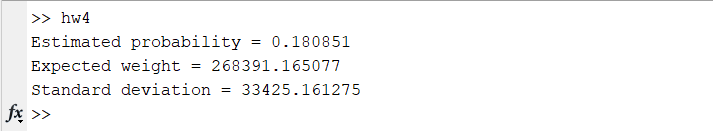
\includegraphics[width=\linewidth]{Screenshot (2317).png}
    \caption*{Printed Result of the Code Above}
  \end{subfigure}
\end{figure}


\subsection*{a)} 
$-$ The estimated probability is 0.180851, so we can understand that approximately $18\%$ of the time  the total weight of the cargo unloaded at the port in a day exceeds the target weight of 300000 tons. Since, this is a Monte Carlo Simulation, if we want a superior precision for our estimator, we must increase our sample size.\\
\subsection*{b)} 
$-$ The estimated expected total weight is 268391.165077 tons. This is the average weight of all the cargo unloaded at the port in a day. It is essential to keep in mind that this estimate is subject to randomness and uncertainty due to the simulation approach. So, if we increase our sample size, the estimated weight will converge to the real weight.\\
\subsection*{c)} 
$-$ The estimated standard deviation is 33425.161275 tons. This value represents  the variability of the total weight across different Monte Carlo runs. Larger standard deviation values indicate greater variability in the results.\\
\\
$-$ To improve the accuracy of the estimator, we can consider increasing the sample size (N) or adjust the significance level (alpha) and the desired margin of error (epsilon). This way we can get a more precise estimator than the one we have simulated.\\


\end{document}